\documentclass[12pt,]{article}
\usepackage{lmodern}
\usepackage{amssymb,amsmath}
\usepackage{ifxetex,ifluatex}
\usepackage{fixltx2e} % provides \textsubscript
\ifnum 0\ifxetex 1\fi\ifluatex 1\fi=0 % if pdftex
  \usepackage[T1]{fontenc}
  \usepackage[utf8]{inputenc}
\else % if luatex or xelatex
  \ifxetex
    \usepackage{mathspec}
  \else
    \usepackage{fontspec}
  \fi
  \defaultfontfeatures{Ligatures=TeX,Scale=MatchLowercase}
    \setmainfont[]{Times New Roman}
\fi
% use upquote if available, for straight quotes in verbatim environments
\IfFileExists{upquote.sty}{\usepackage{upquote}}{}
% use microtype if available
\IfFileExists{microtype.sty}{%
\usepackage{microtype}
\UseMicrotypeSet[protrusion]{basicmath} % disable protrusion for tt fonts
}{}
\usepackage[margin=2.54cm]{geometry}
\usepackage{hyperref}
\hypersetup{unicode=true,
            pdftitle={Dissolved Organic Carbon in Lakes from the North Temperate Region},
            pdfauthor={Caroline Watson},
            pdfborder={0 0 0},
            breaklinks=true}
\urlstyle{same}  % don't use monospace font for urls
\usepackage{color}
\usepackage{fancyvrb}
\newcommand{\VerbBar}{|}
\newcommand{\VERB}{\Verb[commandchars=\\\{\}]}
\DefineVerbatimEnvironment{Highlighting}{Verbatim}{commandchars=\\\{\}}
% Add ',fontsize=\small' for more characters per line
\usepackage{framed}
\definecolor{shadecolor}{RGB}{248,248,248}
\newenvironment{Shaded}{\begin{snugshade}}{\end{snugshade}}
\newcommand{\KeywordTok}[1]{\textcolor[rgb]{0.13,0.29,0.53}{\textbf{#1}}}
\newcommand{\DataTypeTok}[1]{\textcolor[rgb]{0.13,0.29,0.53}{#1}}
\newcommand{\DecValTok}[1]{\textcolor[rgb]{0.00,0.00,0.81}{#1}}
\newcommand{\BaseNTok}[1]{\textcolor[rgb]{0.00,0.00,0.81}{#1}}
\newcommand{\FloatTok}[1]{\textcolor[rgb]{0.00,0.00,0.81}{#1}}
\newcommand{\ConstantTok}[1]{\textcolor[rgb]{0.00,0.00,0.00}{#1}}
\newcommand{\CharTok}[1]{\textcolor[rgb]{0.31,0.60,0.02}{#1}}
\newcommand{\SpecialCharTok}[1]{\textcolor[rgb]{0.00,0.00,0.00}{#1}}
\newcommand{\StringTok}[1]{\textcolor[rgb]{0.31,0.60,0.02}{#1}}
\newcommand{\VerbatimStringTok}[1]{\textcolor[rgb]{0.31,0.60,0.02}{#1}}
\newcommand{\SpecialStringTok}[1]{\textcolor[rgb]{0.31,0.60,0.02}{#1}}
\newcommand{\ImportTok}[1]{#1}
\newcommand{\CommentTok}[1]{\textcolor[rgb]{0.56,0.35,0.01}{\textit{#1}}}
\newcommand{\DocumentationTok}[1]{\textcolor[rgb]{0.56,0.35,0.01}{\textbf{\textit{#1}}}}
\newcommand{\AnnotationTok}[1]{\textcolor[rgb]{0.56,0.35,0.01}{\textbf{\textit{#1}}}}
\newcommand{\CommentVarTok}[1]{\textcolor[rgb]{0.56,0.35,0.01}{\textbf{\textit{#1}}}}
\newcommand{\OtherTok}[1]{\textcolor[rgb]{0.56,0.35,0.01}{#1}}
\newcommand{\FunctionTok}[1]{\textcolor[rgb]{0.00,0.00,0.00}{#1}}
\newcommand{\VariableTok}[1]{\textcolor[rgb]{0.00,0.00,0.00}{#1}}
\newcommand{\ControlFlowTok}[1]{\textcolor[rgb]{0.13,0.29,0.53}{\textbf{#1}}}
\newcommand{\OperatorTok}[1]{\textcolor[rgb]{0.81,0.36,0.00}{\textbf{#1}}}
\newcommand{\BuiltInTok}[1]{#1}
\newcommand{\ExtensionTok}[1]{#1}
\newcommand{\PreprocessorTok}[1]{\textcolor[rgb]{0.56,0.35,0.01}{\textit{#1}}}
\newcommand{\AttributeTok}[1]{\textcolor[rgb]{0.77,0.63,0.00}{#1}}
\newcommand{\RegionMarkerTok}[1]{#1}
\newcommand{\InformationTok}[1]{\textcolor[rgb]{0.56,0.35,0.01}{\textbf{\textit{#1}}}}
\newcommand{\WarningTok}[1]{\textcolor[rgb]{0.56,0.35,0.01}{\textbf{\textit{#1}}}}
\newcommand{\AlertTok}[1]{\textcolor[rgb]{0.94,0.16,0.16}{#1}}
\newcommand{\ErrorTok}[1]{\textcolor[rgb]{0.64,0.00,0.00}{\textbf{#1}}}
\newcommand{\NormalTok}[1]{#1}
\usepackage{graphicx,grffile}
\makeatletter
\def\maxwidth{\ifdim\Gin@nat@width>\linewidth\linewidth\else\Gin@nat@width\fi}
\def\maxheight{\ifdim\Gin@nat@height>\textheight\textheight\else\Gin@nat@height\fi}
\makeatother
% Scale images if necessary, so that they will not overflow the page
% margins by default, and it is still possible to overwrite the defaults
% using explicit options in \includegraphics[width, height, ...]{}
\setkeys{Gin}{width=\maxwidth,height=\maxheight,keepaspectratio}
\IfFileExists{parskip.sty}{%
\usepackage{parskip}
}{% else
\setlength{\parindent}{0pt}
\setlength{\parskip}{6pt plus 2pt minus 1pt}
}
\setlength{\emergencystretch}{3em}  % prevent overfull lines
\providecommand{\tightlist}{%
  \setlength{\itemsep}{0pt}\setlength{\parskip}{0pt}}
\setcounter{secnumdepth}{5}
% Redefines (sub)paragraphs to behave more like sections
\ifx\paragraph\undefined\else
\let\oldparagraph\paragraph
\renewcommand{\paragraph}[1]{\oldparagraph{#1}\mbox{}}
\fi
\ifx\subparagraph\undefined\else
\let\oldsubparagraph\subparagraph
\renewcommand{\subparagraph}[1]{\oldsubparagraph{#1}\mbox{}}
\fi

%%% Use protect on footnotes to avoid problems with footnotes in titles
\let\rmarkdownfootnote\footnote%
\def\footnote{\protect\rmarkdownfootnote}

%%% Change title format to be more compact
\usepackage{titling}

% Create subtitle command for use in maketitle
\providecommand{\subtitle}[1]{
  \posttitle{
    \begin{center}\large#1\end{center}
    }
}

\setlength{\droptitle}{-2em}

  \title{Dissolved Organic Carbon in Lakes from the North Temperate Region}
    \pretitle{\vspace{\droptitle}\centering\huge}
  \posttitle{\par}
  \subtitle{\url{https://github.com/cwatson1013/Env_Data_Analysis_Final_Proj.git}}
  \author{Caroline Watson}
    \preauthor{\centering\large\emph}
  \postauthor{\par}
    \date{}
    \predate{}\postdate{}
  
\usepackage{booktabs}
\usepackage{longtable}
\usepackage{array}
\usepackage{multirow}
\usepackage{wrapfig}
\usepackage{float}
\usepackage{colortbl}
\usepackage{pdflscape}
\usepackage{tabu}
\usepackage{threeparttable}
\usepackage{threeparttablex}
\usepackage[normalem]{ulem}
\usepackage{makecell}
\usepackage{xcolor}

\begin{document}
\maketitle
\begin{abstract}
Dissolved organic carbon (DOC) is a significant part of the carbon
cycle. DOC can come from within the lake, such as from decaying
organisms or plant matter, or from the catchment area of the lake. The
catchment area soils can influence the amount of DOC that enters each
lake. The purpose of this study is to see if there is a relationship
between depth and DOC and if so, if there is a seasonal relationship.
This study looked at lakes that were part of the North Temperate Region
located in Wisconsin, USA. DOC was found to not be normally distributed,
so a two-way ANOVA with an interaction test was conducted. The results
found that depth and lake name were significant. A non-parametric test
was run on Peter, Paul, and West Long lakes to determine trends and
changepoints in the data. Peter and West Long lake had trends and
changepoints, but Paul lake did not. Overall, it was found that the
depth and DOC do not have a relationship and a seasonal relationship
between change in depth and DOC could not be determined with the data.
\end{abstract}

\newpage

\tableofcontents  \newpage
\listoftables  \newpage
\listoffigures  \newpage

\begin{Shaded}
\begin{Highlighting}[]
\NormalTok{knitr}\OperatorTok{::}\NormalTok{opts_chunk}\OperatorTok{$}\KeywordTok{set}\NormalTok{(}\DataTypeTok{echo =} \OtherTok{TRUE}\NormalTok{, }\DataTypeTok{eval =} \OtherTok{TRUE}\NormalTok{,}
                      \DataTypeTok{cache =} \OtherTok{TRUE}\NormalTok{, }\DataTypeTok{fig.pos =} \StringTok{"H"}\NormalTok{, }\DataTypeTok{warning =} \OtherTok{FALSE}\NormalTok{, }\DataTypeTok{message =} \OtherTok{FALSE}\NormalTok{)}

\CommentTok{# Set your working directory}
\KeywordTok{setwd}\NormalTok{(}\StringTok{"/Users/carolinewatson/Documents/Spring 2019/Environmental Data Analytics/Final_Project/Data/Code"}\NormalTok{)}

\CommentTok{# Load your packages}
\KeywordTok{suppressMessages}\NormalTok{(}\KeywordTok{library}\NormalTok{(tidyverse))}
\KeywordTok{library}\NormalTok{(ggplot2)}
\KeywordTok{library}\NormalTok{(leaflet)}
\KeywordTok{library}\NormalTok{(dplyr)}
\KeywordTok{library}\NormalTok{(RColorBrewer)}
\KeywordTok{library}\NormalTok{(viridis)}
\KeywordTok{library}\NormalTok{(knitr)}
\KeywordTok{library}\NormalTok{(kableExtra)}
\KeywordTok{library}\NormalTok{(lubridate)}
\KeywordTok{library}\NormalTok{(lme4)}
\KeywordTok{library}\NormalTok{(nlme)}
\KeywordTok{library}\NormalTok{(trend)}
\KeywordTok{library}\NormalTok{(gridExtra)}
\KeywordTok{library}\NormalTok{(multcomp)}

\CommentTok{# Set your ggplot theme}
\NormalTok{caroline_theme <-}\StringTok{ }\KeywordTok{theme_classic}\NormalTok{(}\DataTypeTok{base_size =} \DecValTok{16}\NormalTok{) }\OperatorTok{+}\StringTok{ }
\StringTok{  }\KeywordTok{theme}\NormalTok{(}\DataTypeTok{axis.text =} \KeywordTok{element_text}\NormalTok{(}\DataTypeTok{color =} \StringTok{"black"}\NormalTok{), }
        \DataTypeTok{legend.position =} \StringTok{"right"}\NormalTok{)}

\KeywordTok{theme_set}\NormalTok{(caroline_theme)}
\end{Highlighting}
\end{Shaded}

\section{Research Question and
Rationale}\label{research-question-and-rationale}

The rationale for this analysis is that there typically is a
relationship between dissolved organic carbon and depth. There is also
typically a relationship between land area surrounding lakes that have
high amounts of organic soils usually deposit large amounts of dissolved
organic carbon into lakes. Dissolved organic carbon is an important part
of the carbon cycle and supplies nutrients for some organisms. Most DOC
is natural, but high amounts can indicate human influence, such as land
surrounding the lake that is high in organic amount.

This study aims to find out whether there is a relationship between
dissolved organic carbon (DOC) and depth. If there is a relationship
between these two variables, I want to see if this relationship varies
seasonally. This dataset contains various parameter measurements for
different lakes in the North Temperate Region in Wisconsin, USA that
were part of the Long Term Ecological Research station. The measured
parameters include temperature, depth, dissolved organic carbon,
dissolved inorganic carbon, particulate organic matter and others.

\newpage

\section{Dataset Information}\label{dataset-information}

The data for this analysis were collected from June 3, 1984 - August 17,
2016. Dissolved inorganic carbon (DIC), dissolved organic carbon (DOC),
particulate organic matter, partial pressure of CO2, and absorbance at
440nm were all parameters that were measured. Peter, Paul, West Long,
East Long, Tuesday, and Crampton lakes were all sampled. The samples for
dissolved organic carbon and absorbance were collected from the
epilimnion, metalimnion, hypolimnion and PML (Pooled Mixed Layer). It is
important to note that there were no numeric depths corresponding to DOC
or absorbance. The samples for inorganic carbon were taken at 100\%,
50\%, 25\%, 10\%, 5\%, and 1\% of the surface irridance, with some
samples being collected from the hypolimnion as well. Two types of
samples for partial pressure of CO2 were obtained: one was from the air,
the other from the lake. The air sample was taken at 2 meters above the
lake, and the water sample was taken right below the surface of the
lake. from 2 meters above the surface of the lake, Table 1 shows a
summary of all the measurements in the carbon dataset. The frequency of
the sampling varied.

\begin{Shaded}
\begin{Highlighting}[]
\CommentTok{#reading in data file}
\NormalTok{carbon.data <-}\StringTok{ }\KeywordTok{read.csv}\NormalTok{(}\StringTok{"../Raw/NTL-LTER_Lake_Carbon_Raw.csv"}\NormalTok{)}

\CommentTok{#structure of data frame}
\NormalTok{carbon.data.summary <-}\StringTok{ }\KeywordTok{summary}\NormalTok{(carbon.data)}
\end{Highlighting}
\end{Shaded}

\begin{landscape}\begin{table}[!h]

\caption{\label{tab:unnamed-chunk-2}Summary of Carbon Data from NTL-LTER Lakes in Wisconsin}
\centering
\resizebox{\linewidth}{!}{
\begin{tabular}{l|l|l|l|l|l|l|l|l|l|l|l|l|l|l|l}
\hline
  &     lakeid &           lakename &     year4 &     daynum &   sampledate &         depth &    depth\_id &      tpc &      tpn &     DIC\_mg &     DIC\_uM &    air\_pco2 &   water\_pco2 &      doc &   absorbance\\
\hline
\rowcolor{gray!6}   & R      :3887 & Peter Lake    :3887 & Min.   :1984 & Min.   : 82.0 & 5/24/99:   18 & 0          :1719 & Min.   :-2.000 & Min.   : 0.100 & Min.   :0.000 & Min.   : 0.023 & Min.   :   1.917 & Min.   :197.7 & Min.   :   0.0 & Min.   : 2.710 & Min.   :0.011\\
\hline
 & L      :3852 & Paul Lake     :3852 & 1st Qu.:1993 & 1st Qu.:166.0 & 5/25/99:   18 & Metalimnion:1297 & 1st Qu.: 1.000 & 1st Qu.: 0.580 & 1st Qu.:0.070 & 1st Qu.: 0.812 & 1st Qu.:  67.625 & 1st Qu.:343.4 & 1st Qu.: 478.0 & 1st Qu.: 4.570 & 1st Qu.:0.060\\
\hline
\rowcolor{gray!6}   & T      :1818 & Tuesday Lake  :1818 & Median :1999 & Median :192.0 & 5/26/99:   18 & Hypolimnion:1020 & Median : 3.000 & Median : 0.890 & Median :0.103 & Median : 1.322 & Median : 110.167 & Median :362.9 & Median : 838.5 & Median : 5.603 & Median :0.146\\
\hline
 & W      :1571 & West Long Lake:1571 & Mean   :2000 & Mean   :192.4 & 5/31/99:   18 & PML        : 876 & Mean   : 2.775 & Mean   : 1.110 & Mean   :0.149 & Mean   : 2.310 & Mean   : 192.487 & Mean   :360.4 & Mean   :1012.3 & Mean   : 6.932 & Mean   :0.194\\
\hline
\rowcolor{gray!6}   & E      :1435 & East Long Lake:1435 & 3rd Qu.:2007 & 3rd Qu.:218.0 & 6/1/99 :   18 & Epilimnion : 570 & 3rd Qu.: 5.000 & 3rd Qu.: 1.305 & 3rd Qu.:0.180 & 3rd Qu.: 1.968 & 3rd Qu.: 164.000 & 3rd Qu.:379.0 & 3rd Qu.:1175.6 & 3rd Qu.: 8.370 & 3rd Qu.:0.265\\
\hline
 & M      : 456 & Crampton Lake : 456 & Max.   :2016 & Max.   :310.0 & 6/14/99:   18 & (Other)    :7918 & Max.   : 7.000 & Max.   :11.860 & Max.   :2.170 & Max.   :48.599 & Max.   :4049.883 & Max.   :608.1 & Max.   :9348.2 & Max.   :44.080 & Max.   :1.213\\
\hline
\rowcolor{gray!6}   & (Other): 538 & (Other)       : 538 & NA & NA & (Other):13449 & NA's       : 157 & NA's   :170 & NA's   :11410 & NA's   :11409 & NA's   :3642 & NA's   :3642 & NA's   :12411 & NA's   :12411 & NA's   :9993 & NA's   :10658\\
\hline
\end{tabular}}
\end{table}
\end{landscape}

\newpage

\section{Exploratory Data Analysis and
Wrangling}\label{exploratory-data-analysis-and-wrangling}

\begin{Shaded}
\begin{Highlighting}[]
\CommentTok{#class of sampledate column}
\KeywordTok{class}\NormalTok{(carbon.data}\OperatorTok{$}\NormalTok{sampledate)}
\end{Highlighting}
\end{Shaded}

\begin{verbatim}
## [1] "factor"
\end{verbatim}

\begin{Shaded}
\begin{Highlighting}[]
\CommentTok{#converting sampledate to a date in R}
\NormalTok{carbon.data}\OperatorTok{$}\NormalTok{sampledate <-}\StringTok{ }\KeywordTok{as.Date}\NormalTok{(carbon.data}\OperatorTok{$}\NormalTok{sampledate, }\DataTypeTok{format =} \StringTok{"%m/%d/%y"}\NormalTok{)}

\CommentTok{#checking class of sampledate}
\KeywordTok{class}\NormalTok{(carbon.data}\OperatorTok{$}\NormalTok{sampledate)}
\end{Highlighting}
\end{Shaded}

\begin{verbatim}
## [1] "Date"
\end{verbatim}

\begin{Shaded}
\begin{Highlighting}[]
\CommentTok{#summary of the dataset}
\KeywordTok{head}\NormalTok{(carbon.data)}
\end{Highlighting}
\end{Shaded}

\begin{verbatim}
##   lakeid   lakename year4 daynum sampledate depth depth_id tpc tpn DIC_mg
## 1      L  Paul Lake  1984    155 1984-06-03     0        1  NA  NA   1.45
## 2      L  Paul Lake  1984    155 1984-06-03     1        2  NA  NA   1.82
## 3      L  Paul Lake  1984    155 1984-06-03     2        3  NA  NA   1.51
## 4      L  Paul Lake  1984    155 1984-06-03   3.5        4  NA  NA   1.47
## 5      L  Paul Lake  1984    155 1984-06-03   5.5        5  NA  NA   2.69
## 6      R Peter Lake  1984    156 1984-06-04     0        1  NA  NA   2.85
##     DIC_uM air_pco2 water_pco2 doc absorbance
## 1 120.8333       NA         NA  NA         NA
## 2 151.6667       NA         NA  NA         NA
## 3 125.8333       NA         NA  NA         NA
## 4 122.5000       NA         NA  NA         NA
## 5 224.1667       NA         NA  NA         NA
## 6 237.5000       NA         NA  NA         NA
\end{verbatim}

\begin{Shaded}
\begin{Highlighting}[]
\KeywordTok{summary}\NormalTok{(carbon.data)}
\end{Highlighting}
\end{Shaded}

\begin{verbatim}
##      lakeid               lakename        year4          daynum     
##  R      :3887   Peter Lake    :3887   Min.   :1984   Min.   : 82.0  
##  L      :3852   Paul Lake     :3852   1st Qu.:1993   1st Qu.:166.0  
##  T      :1818   Tuesday Lake  :1818   Median :1999   Median :192.0  
##  W      :1571   West Long Lake:1571   Mean   :2000   Mean   :192.4  
##  E      :1435   East Long Lake:1435   3rd Qu.:2007   3rd Qu.:218.0  
##  M      : 456   Crampton Lake : 456   Max.   :2016   Max.   :310.0  
##  (Other): 538   (Other)       : 538                                 
##    sampledate                 depth         depth_id           tpc        
##  Min.   :1984-06-03   0          :1719   Min.   :-2.000   Min.   : 0.100  
##  1st Qu.:1993-06-16   Metalimnion:1297   1st Qu.: 1.000   1st Qu.: 0.580  
##  Median :1999-07-06   Hypolimnion:1020   Median : 3.000   Median : 0.890  
##  Mean   :2000-07-14   PML        : 876   Mean   : 2.775   Mean   : 1.110  
##  3rd Qu.:2007-08-28   Epilimnion : 570   3rd Qu.: 5.000   3rd Qu.: 1.305  
##  Max.   :2016-08-17   (Other)    :7918   Max.   : 7.000   Max.   :11.860  
##                       NA's       : 157   NA's   :170      NA's   :11410   
##       tpn            DIC_mg           DIC_uM            air_pco2    
##  Min.   :0.000   Min.   : 0.023   Min.   :   1.917   Min.   :197.7  
##  1st Qu.:0.070   1st Qu.: 0.812   1st Qu.:  67.625   1st Qu.:343.4  
##  Median :0.103   Median : 1.322   Median : 110.167   Median :362.9  
##  Mean   :0.149   Mean   : 2.310   Mean   : 192.487   Mean   :360.4  
##  3rd Qu.:0.180   3rd Qu.: 1.968   3rd Qu.: 164.000   3rd Qu.:379.0  
##  Max.   :2.170   Max.   :48.599   Max.   :4049.883   Max.   :608.1  
##  NA's   :11409   NA's   :3642     NA's   :3642       NA's   :12411  
##    water_pco2          doc           absorbance   
##  Min.   :   0.0   Min.   : 2.710   Min.   :0.011  
##  1st Qu.: 478.0   1st Qu.: 4.570   1st Qu.:0.060  
##  Median : 838.5   Median : 5.603   Median :0.146  
##  Mean   :1012.3   Mean   : 6.932   Mean   :0.194  
##  3rd Qu.:1175.6   3rd Qu.: 8.370   3rd Qu.:0.265  
##  Max.   :9348.2   Max.   :44.080   Max.   :1.213  
##  NA's   :12411    NA's   :9993     NA's   :10658
\end{verbatim}

\begin{Shaded}
\begin{Highlighting}[]
\KeywordTok{colnames}\NormalTok{(carbon.data)}
\end{Highlighting}
\end{Shaded}

\begin{verbatim}
##  [1] "lakeid"     "lakename"   "year4"      "daynum"     "sampledate"
##  [6] "depth"      "depth_id"   "tpc"        "tpn"        "DIC_mg"    
## [11] "DIC_uM"     "air_pco2"   "water_pco2" "doc"        "absorbance"
\end{verbatim}

\begin{Shaded}
\begin{Highlighting}[]
\KeywordTok{dim}\NormalTok{(carbon.data)}
\end{Highlighting}
\end{Shaded}

\begin{verbatim}
## [1] 13557    15
\end{verbatim}

\begin{Shaded}
\begin{Highlighting}[]
\CommentTok{#renaming columns}
\KeywordTok{colnames}\NormalTok{(carbon.data)[}\DecValTok{1}\OperatorTok{:}\DecValTok{5}\NormalTok{] <-}\StringTok{ }\KeywordTok{c}\NormalTok{(}\StringTok{"Lake.ID"}\NormalTok{, }\StringTok{"Lake.Name"}\NormalTok{, }\StringTok{"Year"}\NormalTok{, }\StringTok{"Day.Number"}\NormalTok{, }\StringTok{"Date"}\NormalTok{)}
\end{Highlighting}
\end{Shaded}

The dataset was imported and the date column was formatted as a date in
R. A summary of the dataset was run to understand what the dataset
contained. The head of the dataset was viewed as well as the dimensions
and column names. Some column names were changed to make it easier to
identify them.

\begin{Shaded}
\begin{Highlighting}[]
\CommentTok{#wrangling dataset}
\NormalTok{carbon.data.skinny <-}\StringTok{ }\NormalTok{carbon.data }\OperatorTok
\StringTok{  }\KeywordTok{filter}\NormalTok{(depth_id }\OperatorTok{==}\StringTok{ }\OperatorTok{-}\DecValTok{2} \OperatorTok{|}\StringTok{ }\NormalTok{depth_id }\OperatorTok{==}\StringTok{ }\OperatorTok{-}\DecValTok{1} \OperatorTok{|}\StringTok{ }\NormalTok{depth_id }\OperatorTok{==}\StringTok{ }\DecValTok{7}\NormalTok{) }\OperatorTok
\StringTok{  }\KeywordTok{filter}\NormalTok{(depth }\OperatorTok{==}\StringTok{ "Hypolimnion"} \OperatorTok{|}\StringTok{ }\NormalTok{depth }\OperatorTok{==}\StringTok{ "Epilimnion"} \OperatorTok{|}\StringTok{ }\NormalTok{depth }\OperatorTok{==}\StringTok{ "PML"} \OperatorTok{|}
\StringTok{           }\NormalTok{depth }\OperatorTok{==}\StringTok{ "Metalimnion"}\NormalTok{) }\OperatorTok
\StringTok{  }\KeywordTok{mutate}\NormalTok{(}\DataTypeTok{depth =} \KeywordTok{factor}\NormalTok{(depth, }\DataTypeTok{levels =} \KeywordTok{c}\NormalTok{(}\StringTok{"Epilimnion"}\NormalTok{, }\StringTok{"Metalimnion"}\NormalTok{,}
                                          \StringTok{"PML"}\NormalTok{, }\StringTok{"Hypolimnion"}\NormalTok{))) }\OperatorTok
\StringTok{  }\KeywordTok{filter}\NormalTok{(}\KeywordTok{is.na}\NormalTok{(doc) }\OperatorTok{==}\StringTok{ }\OtherTok{FALSE}\NormalTok{) }\OperatorTok
\StringTok{  }\NormalTok{dplyr}\OperatorTok{::}\KeywordTok{select}\NormalTok{(Lake.ID}\OperatorTok{:}\NormalTok{depth_id, doc)}

\CommentTok{#saving processed file to the processed folder}
\KeywordTok{write.csv}\NormalTok{(carbon.data.skinny, }
          \DataTypeTok{file =} \StringTok{"../Processed/NTL-LTER_Lake_Carbon_Processed.csv"}\NormalTok{)}
\end{Highlighting}
\end{Shaded}

The dataset was wrangled by filtering for depth id and depth
description. DOC measurements were only taken at the epilimnion,
metalimnion, PML, and hypolimnion, so the dataset needed to be filtered
by these options. This study focused mainly on DOC and depth, so columns
such as total particulate carbon, or irridance, were not needed. Columns
that were needed were selected when the data was wrangled. The depths
were also mututated as factor levels so that future analyses would
present the depths from shallowest to deepest (epilimnion to
hypolimnion).

\begin{figure}
\centering
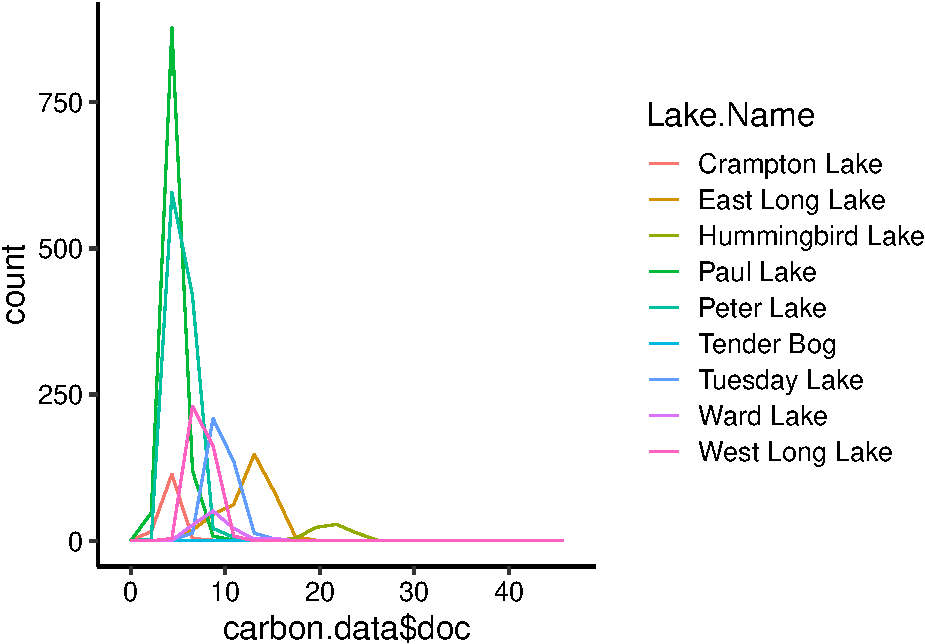
\includegraphics{Watson_ENV872_Project_files/figure-latex/unnamed-chunk-5-1.pdf}
\caption{\label{fig:fig1}QQplot showing whether data for DOC is normally
distributed.}
\end{figure}

\begin{figure}
\centering
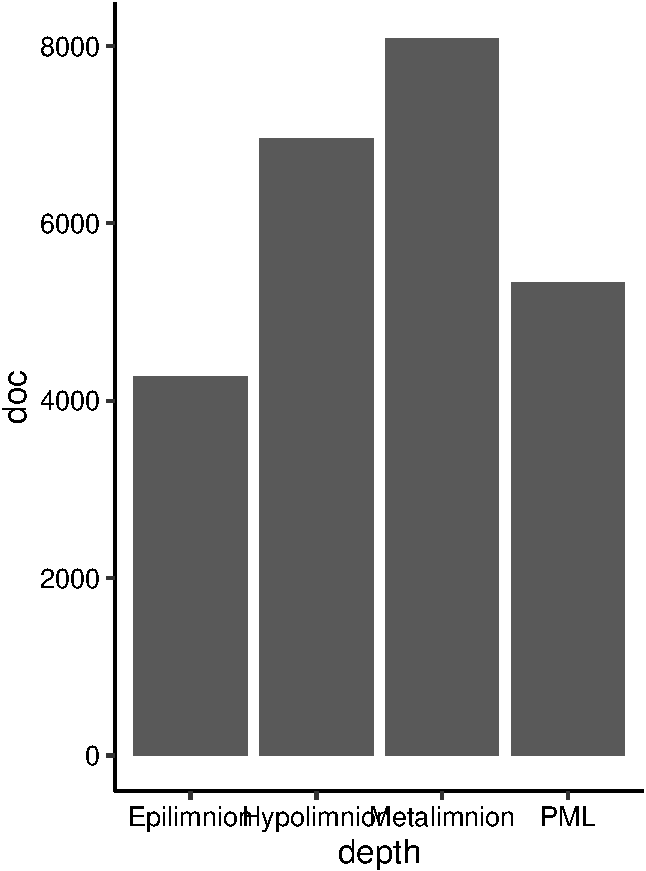
\includegraphics{Watson_ENV872_Project_files/figure-latex/unnamed-chunk-6-1.pdf}
\caption{\label{fig:fig2}Log QQplot of dissolved organic carbon data.}
\end{figure}

\autoref{fig:fig1} is a qqplot that shows whether the dissolved organic
carbon data has a normal distribution. From \autoref{fig:fig1}, it is
clear that the dissolved organic carbon data do not follow a normal
distribution. Becuase the data are not normally distributed, a log
qqplot was run to see if log transforming the data would help the data
look more normally distributed. \autoref{fig:fig2} shows the dissolved
organic carbon data log transformed. From \autoref{fig:fig2} it is clear
that dissolved organic carbon is not normally distributed, but log
transforming the data makes the data more normally distributed than not
log transforming the data.

\begin{figure}
\centering
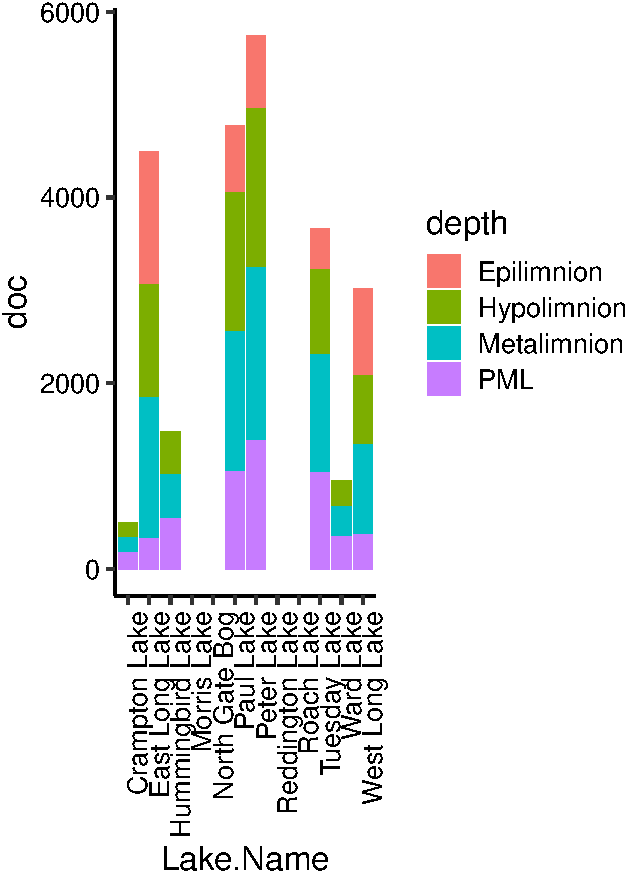
\includegraphics{Watson_ENV872_Project_files/figure-latex/unnamed-chunk-7-1.pdf}
\caption{\label{fig:fig3}Histogram of dissolved organic carbon (mg/L).}
\end{figure}

\autoref{fig:fig3} shows a histogram of the distribution of dissolved
organic carbon (mg/L). From \autoref{fig:fig3} it is apparent that the
distribution of dissolved organic carbon is not noramlly distributed.
This information will factor into the statistical analyses conducted
since the data is not normally distributed.

\begin{figure}
\centering
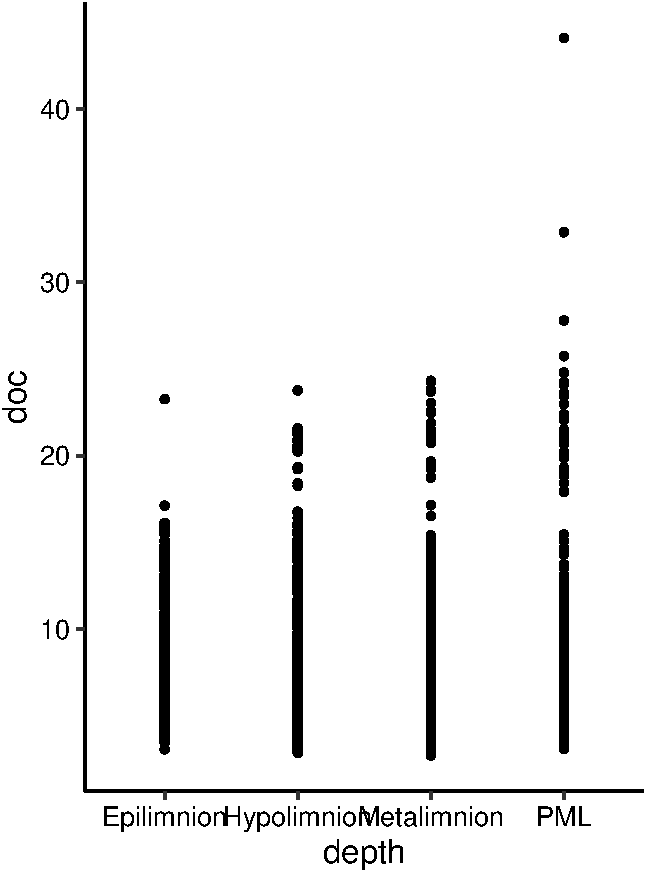
\includegraphics{Watson_ENV872_Project_files/figure-latex/unnamed-chunk-8-1.pdf}
\caption{\label{fig:fig4}Frequency Polygon showing the count of DOC
(mg/L) amounts in each Lake}
\end{figure}

\autoref{fig:fig4} shows the cumulative frequency of dissolved organice
carbon in each lake. From \autoref{fig:fig4}, it is apparent that Paul
lake has the highest cumulative frequency of dissolved organic carbon,
followed by Peter lake. \autoref{fig:fig4} also shows that Peter and
Paul lake mainly have dissolved organic carbon amounts between 0 mg/L
and 10 mg/L, which is why there are two high spikes. The other lakes
have dissolved orgnic carbon amounts that are more spread out, as shown
in \autoref{fig:fig4}.

\begin{figure}
\centering
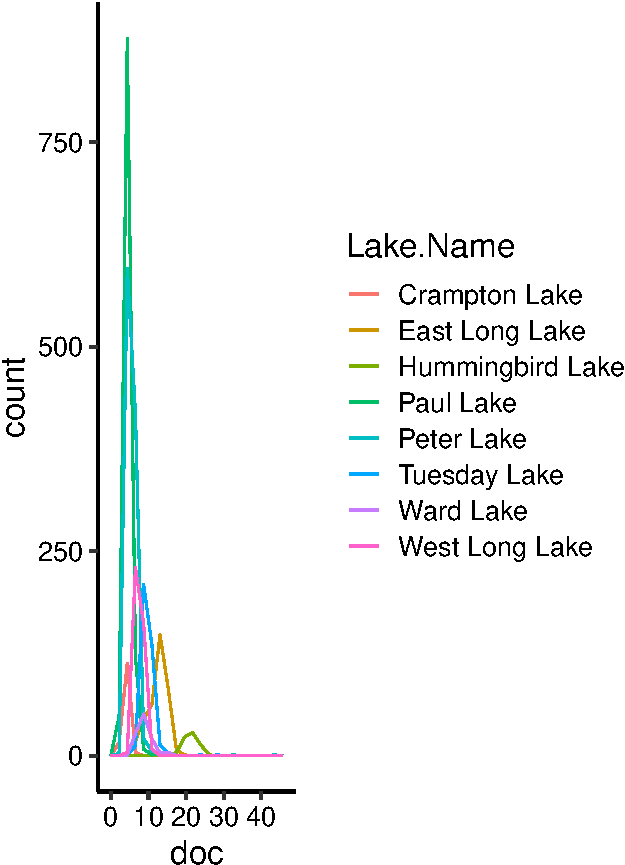
\includegraphics{Watson_ENV872_Project_files/figure-latex/unnamed-chunk-9-1.pdf}
\caption{\label{fig:fig5} Dissolved Organic Carbon varying with depth.
Depth increases from left to right, with Epilimnion being the surface of
the lake.}
\end{figure}

\autoref{fig:fig5} shows a box plot of each depth category of the lake
against the doc measurements. From \autoref{fig:fig5} it looks like
there is no relationship between depth and dissolved organic carbon
(mg/L). \autoref{fig:fig5} indicates that the Epilimnion (water closest
to the surface) and Hypolimnion (water from deepest part of the lake)
have greater medians than the Metalimnion or the pooled mixed layer
(PML). However, the PML has the greatest distribution of dissolved
organic carbon, with one sample that might be considered an outlier as
seen in \autoref{fig:fig5}.

\begin{figure}
\centering
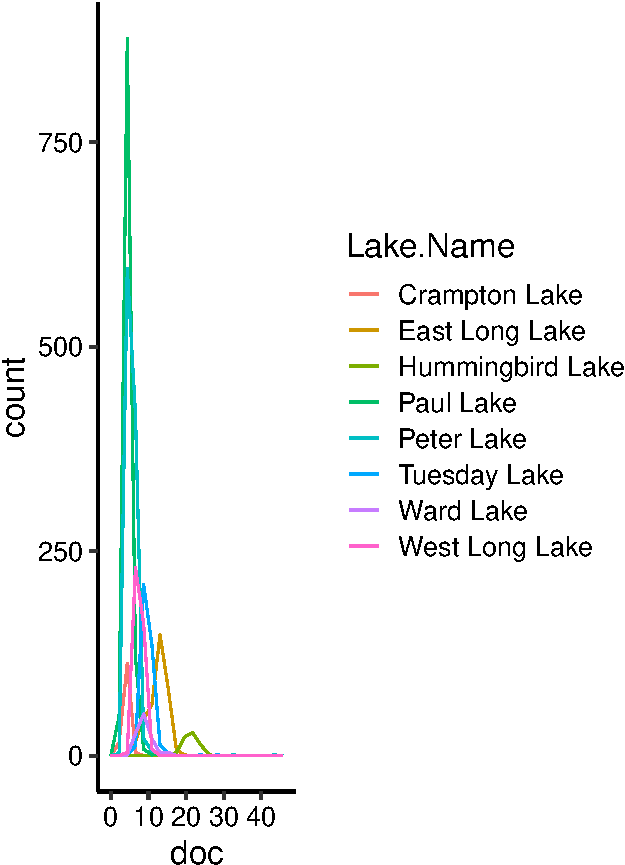
\includegraphics{Watson_ENV872_Project_files/figure-latex/unnamed-chunk-10-1.pdf}
\caption{\label{fig:fig6}Distribution of dissolved organic carbon (mg/L)
in each depth faceted by lake.}
\end{figure}

\autoref{fig:fig6} shows the distribution of dissolved organic carbon
(mg/L) in each depth layer faceted by each lake. From
\autoref{fig:fig6}, the PML of Peter lake has the greatest distribution
of dissolved organic carbon (mg/L). Further, the distribution of
dissolved organic carbon (mg/L) in each lake does not vary with depth.

\begin{figure}
\centering
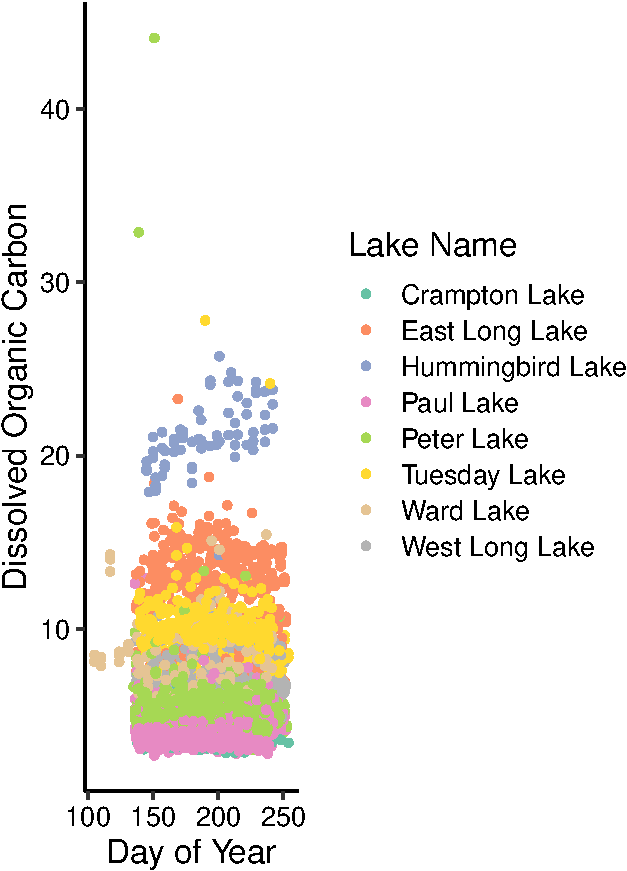
\includegraphics{Watson_ENV872_Project_files/figure-latex/unnamed-chunk-11-1.pdf}
\caption{\label{fig:fig7} Dissolved organic carbon (mg/L) over time in
each lake.}
\end{figure}

\autoref{fig:fig7} shows dissolved organic carbon over the years.
\autoref{fig:fig1} was created to determine if there was a pattern of
dissolved organic carbon in lakes over the years. From
\autoref{fig:fig7} only Peter, Paul, and West long lake were
continuously sampled very year. Other lakes, such as Hummingbird lake,
were only sampled between the late 1990s to the early 2000s.

\begin{figure}
\centering
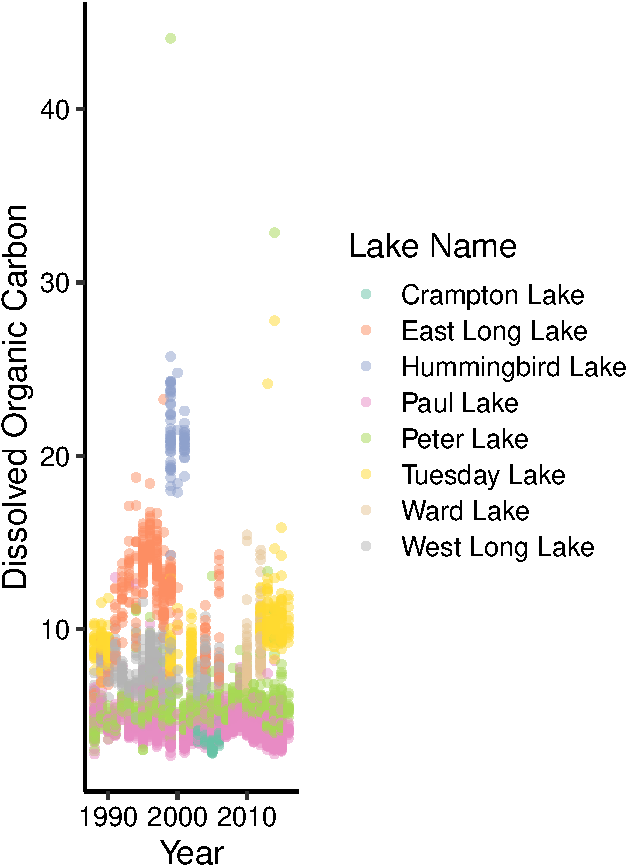
\includegraphics{Watson_ENV872_Project_files/figure-latex/unnamed-chunk-12-1.pdf}
\caption{\label{fig:fig8} Dissolved organic carbon (mg/L) by day of the
year.}
\end{figure}

\autoref{fig:fig8} shows the day number of the year plotted against
dissolved organic carbon (mg/L) with different colors for each lake.
From \autoref{fig:fig8} it is apparent that sampling was done mainly
between days 140 and 250 of the year, which is during spring and summer
months. Since samples were taken during the spring and summer months, it
will not be possible to analyze whether DOC varies with depth
seasonally.

\newpage

\section{Analysis}\label{analysis}

\begin{Shaded}
\begin{Highlighting}[]
\CommentTok{#Shapiro-Wilkes test for normality}
\KeywordTok{shapiro.test}\NormalTok{(carbon.data.skinny}\OperatorTok{$}\NormalTok{doc)}
\end{Highlighting}
\end{Shaded}

\begin{verbatim}
## 
##  Shapiro-Wilk normality test
## 
## data:  carbon.data.skinny$doc
## W = 0.79256, p-value < 2.2e-16
\end{verbatim}

\begin{Shaded}
\begin{Highlighting}[]
\CommentTok{#Bartlett test for equal variance}
\KeywordTok{bartlett.test}\NormalTok{(carbon.data.skinny}\OperatorTok{$}\NormalTok{doc, carbon.data.skinny}\OperatorTok{$}\NormalTok{depth, }
\NormalTok{              carbon.data.skinny}\OperatorTok{$}\NormalTok{Lake.Name)}
\end{Highlighting}
\end{Shaded}

\begin{verbatim}
## 
##  Bartlett test of homogeneity of variances
## 
## data:  carbon.data.skinny$doc and carbon.data.skinny$depth
## Bartlett's K-squared = 53.202, df = 3, p-value = 1.66e-11
\end{verbatim}

\begin{Shaded}
\begin{Highlighting}[]
\CommentTok{#Interaction effects with two-way ANOVA}
\NormalTok{carbon_aov <-}\StringTok{ }\KeywordTok{aov}\NormalTok{(}\DataTypeTok{data =}\NormalTok{ carbon.data.skinny, doc }\OperatorTok{~}\StringTok{ }\NormalTok{depth}\OperatorTok{*}\NormalTok{Lake.Name)}
\KeywordTok{summary}\NormalTok{(carbon_aov)}
\end{Highlighting}
\end{Shaded}

\begin{verbatim}
##                   Df Sum Sq Mean Sq F value Pr(>F)    
## depth              3    501     167   72.95 <2e-16 ***
## Lake.Name          7  37637    5377 2346.86 <2e-16 ***
## depth:Lake.Name   18    612      34   14.84 <2e-16 ***
## Residuals       3529   8085       2                   
## ---
## Signif. codes:  0 '***' 0.001 '**' 0.01 '*' 0.05 '.' 0.1 ' ' 1
\end{verbatim}

\begin{Shaded}
\begin{Highlighting}[]
\CommentTok{#Interaction effects with two-way ANOVA with log of DOC}
\NormalTok{carbon_aov_log <-}\StringTok{ }\KeywordTok{aov}\NormalTok{(}\DataTypeTok{data =}\NormalTok{ carbon.data.skinny, }\KeywordTok{log}\NormalTok{(doc) }\OperatorTok{~}\StringTok{ }\NormalTok{depth}\OperatorTok{*}\NormalTok{Lake.Name)}
\KeywordTok{summary}\NormalTok{(carbon_aov_log) }
\end{Highlighting}
\end{Shaded}

\begin{verbatim}
##                   Df Sum Sq Mean Sq F value Pr(>F)    
## depth              3   16.0    5.34  193.33 <2e-16 ***
## Lake.Name          7  528.5   75.50 2735.83 <2e-16 ***
## depth:Lake.Name   18   10.9    0.61   21.93 <2e-16 ***
## Residuals       3529   97.4    0.03                   
## ---
## Signif. codes:  0 '***' 0.001 '**' 0.01 '*' 0.05 '.' 0.1 ' ' 1
\end{verbatim}

\begin{Shaded}
\begin{Highlighting}[]
\CommentTok{#post-hoc Tukey test using the glht function}
\NormalTok{K <-}\StringTok{ }\KeywordTok{diag}\NormalTok{(}\KeywordTok{length}\NormalTok{(}\KeywordTok{coef}\NormalTok{(carbon_aov)))[}\OperatorTok{-}\DecValTok{1}\NormalTok{,] }
\KeywordTok{rownames}\NormalTok{(K) <-}\StringTok{ }\KeywordTok{names}\NormalTok{(}\KeywordTok{coef}\NormalTok{(carbon_aov))[}\OperatorTok{-}\DecValTok{1}\NormalTok{]}

\NormalTok{carbon.data.skinny}\OperatorTok{$}\NormalTok{dl <-}\StringTok{ }\KeywordTok{with}\NormalTok{(carbon.data.skinny, }\KeywordTok{interaction}\NormalTok{(depth, Lake.Name))}
\NormalTok{cell <-}\StringTok{ }\KeywordTok{aov}\NormalTok{(doc }\OperatorTok{~}\StringTok{ }\NormalTok{dl }\OperatorTok{-}\StringTok{ }\DecValTok{1}\NormalTok{, }\DataTypeTok{data =}\NormalTok{ carbon.data.skinny)}
\NormalTok{carbon.tukey <-}\StringTok{ }\KeywordTok{summary}\NormalTok{(}\KeywordTok{glht}\NormalTok{(cell, }\DataTypeTok{linfct =}\NormalTok{ K))}
\NormalTok{carbon.tukey}
\end{Highlighting}
\end{Shaded}

\begin{verbatim}
## 
##   Simultaneous Tests for General Linear Hypotheses
## 
## Fit: aov(formula = doc ~ dl - 1, data = carbon.data.skinny)
## 
## Linear Hypotheses:
##                                                 Estimate Std. Error
## depthMetalimnion == 0                            4.01891    0.22317
## depthPML == 0                                    3.65628    0.23082
## depthHypolimnion == 0                           12.09644    0.13934
## Lake.NameEast Long Lake == 0                    12.20887    0.13593
## Lake.NameHummingbird Lake == 0                  10.30667    0.26349
## Lake.NamePaul Lake == 0                         13.52778    0.15955
## Lake.NamePeter Lake == 0                        21.67227    0.32270
## Lake.NameTuesday Lake == 0                      21.33154    0.29684
## Lake.NameWard Lake == 0                         20.33227    0.32270
## Lake.NameWest Long Lake == 0                     5.02601    0.12658
## depthMetalimnion:Lake.NameEast Long Lake == 0    4.03800    0.07837
## depthPML:Lake.NameEast Long Lake == 0            4.28410    0.09592
## depthHypolimnion:Lake.NameEast Long Lake == 0    5.11462    0.08873
## depthMetalimnion:Lake.NameHummingbird Lake == 0  5.42785    0.12613
## depthPML:Lake.NameHummingbird Lake == 0          5.04127    0.07869
## depthMetalimnion:Lake.NamePaul Lake == 0         5.70222    0.09670
## depthPML:Lake.NamePaul Lake == 0                 5.89853    0.08904
## depthHypolimnion:Lake.NamePaul Lake == 0         8.97809    0.22078
## depthMetalimnion:Lake.NamePeter Lake == 0        9.40004    0.13027
## depthPML:Lake.NamePeter Lake == 0                9.99247    0.14771
## depthHypolimnion:Lake.NamePeter Lake == 0       10.37263    0.16044
## depthMetalimnion:Lake.NameTuesday Lake == 0      8.81972    0.25227
## depthPML:Lake.NameTuesday Lake == 0             10.08417    0.25227
## depthHypolimnion:Lake.NameTuesday Lake == 0      7.67629    0.25585
## depthMetalimnion:Lake.NameWard Lake == 0         7.84966    0.13934
## depthPML:Lake.NameWard Lake == 0                 7.12182    0.12932
## depthMetalimnion:Lake.NameWest Long Lake == 0    8.25478    0.22317
## depthPML:Lake.NameWest Long Lake == 0            7.30373    0.14987
##                                                 t value Pr(>|t|)    
## depthMetalimnion == 0                             18.01   <2e-16 ***
## depthPML == 0                                     15.84   <2e-16 ***
## depthHypolimnion == 0                             86.81   <2e-16 ***
## Lake.NameEast Long Lake == 0                      89.82   <2e-16 ***
## Lake.NameHummingbird Lake == 0                    39.12   <2e-16 ***
## Lake.NamePaul Lake == 0                           84.79   <2e-16 ***
## Lake.NamePeter Lake == 0                          67.16   <2e-16 ***
## Lake.NameTuesday Lake == 0                        71.86   <2e-16 ***
## Lake.NameWard Lake == 0                           63.01   <2e-16 ***
## Lake.NameWest Long Lake == 0                      39.71   <2e-16 ***
## depthMetalimnion:Lake.NameEast Long Lake == 0     51.52   <2e-16 ***
## depthPML:Lake.NameEast Long Lake == 0             44.66   <2e-16 ***
## depthHypolimnion:Lake.NameEast Long Lake == 0     57.64   <2e-16 ***
## depthMetalimnion:Lake.NameHummingbird Lake == 0   43.03   <2e-16 ***
## depthPML:Lake.NameHummingbird Lake == 0           64.07   <2e-16 ***
## depthMetalimnion:Lake.NamePaul Lake == 0          58.97   <2e-16 ***
## depthPML:Lake.NamePaul Lake == 0                  66.25   <2e-16 ***
## depthHypolimnion:Lake.NamePaul Lake == 0          40.66   <2e-16 ***
## depthMetalimnion:Lake.NamePeter Lake == 0         72.16   <2e-16 ***
## depthPML:Lake.NamePeter Lake == 0                 67.65   <2e-16 ***
## depthHypolimnion:Lake.NamePeter Lake == 0         64.65   <2e-16 ***
## depthMetalimnion:Lake.NameTuesday Lake == 0       34.96   <2e-16 ***
## depthPML:Lake.NameTuesday Lake == 0               39.97   <2e-16 ***
## depthHypolimnion:Lake.NameTuesday Lake == 0       30.00   <2e-16 ***
## depthMetalimnion:Lake.NameWard Lake == 0          56.34   <2e-16 ***
## depthPML:Lake.NameWard Lake == 0                  55.07   <2e-16 ***
## depthMetalimnion:Lake.NameWest Long Lake == 0     36.99   <2e-16 ***
## depthPML:Lake.NameWest Long Lake == 0             48.73   <2e-16 ***
## ---
## Signif. codes:  0 '***' 0.001 '**' 0.01 '*' 0.05 '.' 0.1 ' ' 1
## (Adjusted p values reported -- single-step method)
\end{verbatim}

\begin{figure}
\centering
\includegraphics{Watson_ENV872_Project_files/figure-latex/unnamed-chunk-14-1.pdf}
\caption{\label{fig:fig9}Plot of Post-Hoc Tukey test showing which
pairwise differences are significant.}
\end{figure}

An interaction effects two-way anova test was run to determine if the
interaction among lake name and depth is significant. The assumptions
are that each variable had been taken independently of the other, that
the data was taken from a normally distributed population, and that the
variances in each group are equal. From \autoref{fig:fig1}, the data
shown is not normally distributed, which thus violates the assumption of
normality. Further, a Shapiro-Wilkes test was run to evaluate whether
the dissolved organic carbon data is well approximated by a normal
distribution. The Shapiro-Wilkes test showed that the data is not well
approximated by a normal distribution (p \textless{} 2.2e-16). A
Bartlett test was run on dissolved organic carbon, lake name, and depth
to see if the variances were equal or different. The Bartlett test had a
p-value less than 0.05, thus the null hypothesis is rejected and the
alternate hypothesis that at least two of the variances are not equal.

From the results, the p-value for depth:Lake.Name is less than 0.05
(p-value = \textless{}2.e16), thus indicating that the interaction
between these terms is siginifcant. Additionally the main effect,
dissolved organic carbon, is significant.

A non-parametric Post-Hoc Tukey test was run to determine the pairwise
differences for the interaction since the interaction was significant.
Pairs are in the same group if the p-value is greater than 0.05. From
the Tukey test, the depths and lake names are all significantlly
different. This is further evidenced in \autoref{fig:fig9}.

\begin{Shaded}
\begin{Highlighting}[]
\CommentTok{#wrangling dataset down to just the three lakes}
\NormalTok{Carbon.three.lakes <-}\StringTok{ }
\StringTok{  }\NormalTok{carbon.data.skinny }\OperatorTok
\StringTok{  }\KeywordTok{filter}\NormalTok{(depth }\OperatorTok{==}\StringTok{ "Hypolimnion"}\NormalTok{) }\OperatorTok
\StringTok{  }\KeywordTok{filter}\NormalTok{(Lake.Name }\OperatorTok{==}\StringTok{ "Peter Lake"} \OperatorTok{|}\StringTok{ }\NormalTok{Lake.Name }\OperatorTok{==}\StringTok{ "Paul Lake"} \OperatorTok{|}
\StringTok{           }\NormalTok{Lake.Name }\OperatorTok{==}\StringTok{ "West Long Lake"}\NormalTok{)}

\CommentTok{#splitting data sets up into each lake data}
\NormalTok{carbon.peter2 <-}\StringTok{ }\KeywordTok{filter}\NormalTok{(Carbon.three.lakes, Lake.Name }\OperatorTok{==}\StringTok{ "Peter Lake"}\NormalTok{)}

\NormalTok{carbon.paul2 <-}\StringTok{ }\KeywordTok{filter}\NormalTok{(Carbon.three.lakes, Lake.Name }\OperatorTok{==}\StringTok{ "Paul Lake"}\NormalTok{)}

\NormalTok{carbon.west2 <-}\StringTok{ }\KeywordTok{filter}\NormalTok{(Carbon.three.lakes, Lake.Name }\OperatorTok{==}\StringTok{ "West Long Lake"}\NormalTok{)}
\end{Highlighting}
\end{Shaded}

A Mann-Kendall test, which is a non-parametric trend test, was run to
determine if there is a monotonic trend in dissolved organic carbon in
Peter, Paul, and West Long lakes over time. This test was chosen because
there is not a linear trend in DOC over time. These lakes were chosen
based off of the \autoref{fig:fig7} which shows which lakes were
monitored continuously over time. The hypolimnion was chosen because
organic carbon can come from decomposed animals and plants in a lake
which could settle at the bottom of the lake. Assumptions of a
Mann-Kendall test include that methods for collecting data are unbiased,
if there is no trend, the data are independently and identically
distributed, and the measurements represent the true states of the
observations when they were taken. In addition to a Mann-Kendall test,
Pettitt's test were run. Pettitt test is a non-parametric test that can
help determine if there is a change in tendancy and if so, where that
change occurs (known as the changepoint).

\begin{Shaded}
\begin{Highlighting}[]
\CommentTok{#Mann-Kendall test for dissolved organic carbon in each lake}

\CommentTok{#mk.test in Paul Lake}
\KeywordTok{mk.test}\NormalTok{(carbon.paul2}\OperatorTok{$}\NormalTok{doc) }\CommentTok{#high p-value so we accept the null that}
\end{Highlighting}
\end{Shaded}

\begin{verbatim}
## 
##  Mann-Kendall trend test
## 
## data:  carbon.paul2$doc
## z = -1.4088, n = 291, p-value = 0.1589
## alternative hypothesis: true S is not equal to 0
## sample estimates:
##             S          varS           tau 
## -2.338000e+03  2.751939e+06 -5.547057e-02
\end{verbatim}

\begin{Shaded}
\begin{Highlighting}[]
\CommentTok{#there is no trend in data}
\end{Highlighting}
\end{Shaded}

The Mann-Kendall test from Paul Lake shows that there is no trend in the
data since the p-value is greater than 0.05 (p-value = 0.1589).

\begin{Shaded}
\begin{Highlighting}[]
\CommentTok{#peter lake}
\KeywordTok{mk.test}\NormalTok{(carbon.peter2}\OperatorTok{$}\NormalTok{doc) }\CommentTok{#low p-value so reject the null and accept that there is a trend in data}
\end{Highlighting}
\end{Shaded}

\begin{verbatim}
## 
##  Mann-Kendall trend test
## 
## data:  carbon.peter2$doc
## z = 4.1173, n = 289, p-value = 3.833e-05
## alternative hypothesis: true S is not equal to 0
## sample estimates:
##            S         varS          tau 
## 6.761000e+03 2.695648e+06 1.626943e-01
\end{verbatim}

\begin{Shaded}
\begin{Highlighting}[]
\CommentTok{#pettitt test to see where changepoint is}
\KeywordTok{pettitt.test}\NormalTok{(carbon.peter2}\OperatorTok{$}\NormalTok{doc) }\CommentTok{#changepoint is at 167}
\end{Highlighting}
\end{Shaded}

\begin{verbatim}
## 
##  Pettitt's test for single change-point detection
## 
## data:  carbon.peter2$doc
## U* = 9629, p-value = 2.119e-10
## alternative hypothesis: two.sided
## sample estimates:
## probable change point at time K 
##                             167
\end{verbatim}

\begin{Shaded}
\begin{Highlighting}[]
\CommentTok{#mk.test before and after changepoint point}
\KeywordTok{mk.test}\NormalTok{(carbon.peter2}\OperatorTok{$}\NormalTok{doc[}\DecValTok{1}\OperatorTok{:}\DecValTok{166}\NormalTok{]) }\CommentTok{#0.06 is greater than 0.05, }
\end{Highlighting}
\end{Shaded}

\begin{verbatim}
## 
##  Mann-Kendall trend test
## 
## data:  carbon.peter2$doc[1:166]
## z = -1.8351, n = 166, p-value = 0.0665
## alternative hypothesis: true S is not equal to 0
## sample estimates:
##             S          varS           tau 
## -1.315000e+03  5.127363e+05 -9.621737e-02
\end{verbatim}

\begin{Shaded}
\begin{Highlighting}[]
\CommentTok{#so accept that there is no trend in this part of the data}
\KeywordTok{mk.test}\NormalTok{(carbon.peter2}\OperatorTok{$}\NormalTok{doc[}\DecValTok{167}\OperatorTok{:}\DecValTok{289}\NormalTok{]) }\CommentTok{#small p-value so could see a trend here}
\end{Highlighting}
\end{Shaded}

\begin{verbatim}
## 
##  Mann-Kendall trend test
## 
## data:  carbon.peter2$doc[167:289]
## z = -3.1, n = 123, p-value = 0.001935
## alternative hypothesis: true S is not equal to 0
## sample estimates:
##             S          varS           tau 
##  -1419.000000 209236.333333     -0.189301
\end{verbatim}

\begin{Shaded}
\begin{Highlighting}[]
\CommentTok{#pettitt test to see if there is a change point between 167 and 289}
\KeywordTok{pettitt.test}\NormalTok{(carbon.peter2}\OperatorTok{$}\NormalTok{doc[}\DecValTok{167}\OperatorTok{:}\DecValTok{289}\NormalTok{]) }\CommentTok{#changepoint at 167+34 = 201}
\end{Highlighting}
\end{Shaded}

\begin{verbatim}
## 
##  Pettitt's test for single change-point detection
## 
## data:  carbon.peter2$doc[167:289]
## U* = 1578, p-value = 0.0006955
## alternative hypothesis: two.sided
## sample estimates:
## probable change point at time K 
##                              34
\end{verbatim}

\begin{Shaded}
\begin{Highlighting}[]
\CommentTok{#mk.test between 167 and 200 and 201 and 289}
\KeywordTok{mk.test}\NormalTok{(carbon.peter2}\OperatorTok{$}\NormalTok{doc[}\DecValTok{167}\OperatorTok{:}\DecValTok{200}\NormalTok{]) }\CommentTok{#p-value less than 0.05, }
\end{Highlighting}
\end{Shaded}

\begin{verbatim}
## 
##  Mann-Kendall trend test
## 
## data:  carbon.peter2$doc[167:200]
## z = 3.7815, n = 34, p-value = 0.0001559
## alternative hypothesis: true S is not equal to 0
## sample estimates:
##           S        varS         tau 
##  256.000000 4547.333333    0.457553
\end{verbatim}

\begin{Shaded}
\begin{Highlighting}[]
\CommentTok{#so might be another trend point in this area}
\KeywordTok{mk.test}\NormalTok{(carbon.peter2}\OperatorTok{$}\NormalTok{doc[}\DecValTok{201}\OperatorTok{:}\DecValTok{289}\NormalTok{]) }\CommentTok{#p-value greater than 0.05, }
\end{Highlighting}
\end{Shaded}

\begin{verbatim}
## 
##  Mann-Kendall trend test
## 
## data:  carbon.peter2$doc[201:289]
## z = -0.34022, n = 89, p-value = 0.7337
## alternative hypothesis: true S is not equal to 0
## sample estimates:
##            S         varS          tau 
##   -97.000000 79620.333333    -0.024786
\end{verbatim}

\begin{Shaded}
\begin{Highlighting}[]
\CommentTok{#so no trend point in this area}

\CommentTok{#pettitt test between 167 and 200}
\KeywordTok{pettitt.test}\NormalTok{(carbon.peter2}\OperatorTok{$}\NormalTok{doc[}\DecValTok{167}\OperatorTok{:}\DecValTok{200}\NormalTok{]) }\CommentTok{#changepoint at 18+167 = 185}
\end{Highlighting}
\end{Shaded}

\begin{verbatim}
## 
##  Pettitt's test for single change-point detection
## 
## data:  carbon.peter2$doc[167:200]
## U* = 238, p-value = 0.0004497
## alternative hypothesis: two.sided
## sample estimates:
## probable change point at time K 
##                              18
\end{verbatim}

\begin{Shaded}
\begin{Highlighting}[]
\CommentTok{#mk.test between 167:184 and 185:200}
\KeywordTok{mk.test}\NormalTok{(carbon.peter2}\OperatorTok{$}\NormalTok{doc[}\DecValTok{167}\OperatorTok{:}\DecValTok{184}\NormalTok{]) }\CommentTok{#p-value is equal to 1, }
\end{Highlighting}
\end{Shaded}

\begin{verbatim}
## 
##  Mann-Kendall trend test
## 
## data:  carbon.peter2$doc[167:184]
## z = 0, n = 18, p-value = 1
## alternative hypothesis: true S is not equal to 0
## sample estimates:
##    S varS  tau 
##    0  696    0
\end{verbatim}

\begin{Shaded}
\begin{Highlighting}[]
\CommentTok{#so accept the null that there are no more trend points}
\KeywordTok{mk.test}\NormalTok{(carbon.peter2}\OperatorTok{$}\NormalTok{doc[}\DecValTok{185}\OperatorTok{:}\DecValTok{200}\NormalTok{]) }\CommentTok{#p-value is greater than 0.05,}
\end{Highlighting}
\end{Shaded}

\begin{verbatim}
## 
##  Mann-Kendall trend test
## 
## data:  carbon.peter2$doc[185:200]
## z = 0.76538, n = 16, p-value = 0.444
## alternative hypothesis: true S is not equal to 0
## sample estimates:
##        S     varS      tau 
##  18.0000 493.3333   0.1500
\end{verbatim}

\begin{Shaded}
\begin{Highlighting}[]
\CommentTok{#so accept the null that there are no more trends}
\end{Highlighting}
\end{Shaded}

The Mann-Kendall test for Peter Lake detected several trends in the data
and the pettitt tets detected several change points. The changepoints
are visible on \autoref{fig:fig10}.

\begin{Shaded}
\begin{Highlighting}[]
\CommentTok{#Mann-Kendall tests and pettitt tests on West Long Lake to detect trends}
\KeywordTok{mk.test}\NormalTok{(carbon.west2}\OperatorTok{$}\NormalTok{doc)}
\end{Highlighting}
\end{Shaded}

\begin{verbatim}
## 
##  Mann-Kendall trend test
## 
## data:  carbon.west2$doc
## z = -0.31518, n = 102, p-value = 0.7526
## alternative hypothesis: true S is not equal to 0
## sample estimates:
##             S          varS           tau 
## -1.100000e+02  1.196027e+05 -2.138624e-02
\end{verbatim}

\begin{Shaded}
\begin{Highlighting}[]
\KeywordTok{pettitt.test}\NormalTok{(carbon.west2}\OperatorTok{$}\NormalTok{doc) }\CommentTok{#changepoint at 60}
\end{Highlighting}
\end{Shaded}

\begin{verbatim}
## 
##  Pettitt's test for single change-point detection
## 
## data:  carbon.west2$doc
## U* = 1013, p-value = 0.006394
## alternative hypothesis: two.sided
## sample estimates:
## probable change point at time K 
##                              60
\end{verbatim}

\begin{Shaded}
\begin{Highlighting}[]
\KeywordTok{mk.test}\NormalTok{(carbon.west2}\OperatorTok{$}\NormalTok{doc[}\DecValTok{1}\OperatorTok{:}\DecValTok{59}\NormalTok{]) }\CommentTok{#trend detected}
\end{Highlighting}
\end{Shaded}

\begin{verbatim}
## 
##  Mann-Kendall trend test
## 
## data:  carbon.west2$doc[1:59]
## z = 2.4917, n = 59, p-value = 0.01271
## alternative hypothesis: true S is not equal to 0
## sample estimates:
##            S         varS          tau 
## 3.820000e+02 2.338067e+04 2.234572e-01
\end{verbatim}

\begin{Shaded}
\begin{Highlighting}[]
\KeywordTok{mk.test}\NormalTok{(carbon.west2}\OperatorTok{$}\NormalTok{doc[}\DecValTok{60}\OperatorTok{:}\DecValTok{102}\NormalTok{]) }\CommentTok{#trend detected}
\end{Highlighting}
\end{Shaded}

\begin{verbatim}
## 
##  Mann-Kendall trend test
## 
## data:  carbon.west2$doc[60:102]
## z = 4.8254, n = 43, p-value = 1.398e-06
## alternative hypothesis: true S is not equal to 0
## sample estimates:
##            S         varS          tau 
##  462.0000000 9127.3333333    0.5124799
\end{verbatim}

\begin{Shaded}
\begin{Highlighting}[]
\CommentTok{#pettitt test}
\KeywordTok{pettitt.test}\NormalTok{(carbon.west2}\OperatorTok{$}\NormalTok{doc[}\DecValTok{1}\OperatorTok{:}\DecValTok{59}\NormalTok{]) }\CommentTok{#changepoint at 16 + 1 = 17}
\end{Highlighting}
\end{Shaded}

\begin{verbatim}
## 
##  Pettitt's test for single change-point detection
## 
## data:  carbon.west2$doc[1:59]
## U* = 587, p-value = 0.0001005
## alternative hypothesis: two.sided
## sample estimates:
## probable change point at time K 
##                              16
\end{verbatim}

\begin{Shaded}
\begin{Highlighting}[]
\KeywordTok{pettitt.test}\NormalTok{(carbon.west2}\OperatorTok{$}\NormalTok{doc[}\DecValTok{60}\OperatorTok{:}\DecValTok{102}\NormalTok{]) }\CommentTok{#changepoint at 23+60 = 83}
\end{Highlighting}
\end{Shaded}

\begin{verbatim}
## 
##  Pettitt's test for single change-point detection
## 
## data:  carbon.west2$doc[60:102]
## U* = 417, p-value = 5.389e-06
## alternative hypothesis: two.sided
## sample estimates:
## probable change point at time K 
##                              23
\end{verbatim}

\begin{Shaded}
\begin{Highlighting}[]
\CommentTok{#mk.test on carbon west}
\KeywordTok{mk.test}\NormalTok{(carbon.west2}\OperatorTok{$}\NormalTok{doc[}\DecValTok{1}\OperatorTok{:}\DecValTok{16}\NormalTok{]) }\CommentTok{#no trend}
\end{Highlighting}
\end{Shaded}

\begin{verbatim}
## 
##  Mann-Kendall trend test
## 
## data:  carbon.west2$doc[1:16]
## z = 0.22511, n = 16, p-value = 0.8219
## alternative hypothesis: true S is not equal to 0
## sample estimates:
##        S     varS      tau 
##   6.0000 493.3333   0.0500
\end{verbatim}

\begin{Shaded}
\begin{Highlighting}[]
\KeywordTok{mk.test}\NormalTok{(carbon.west2}\OperatorTok{$}\NormalTok{doc[}\DecValTok{17}\OperatorTok{:}\DecValTok{59}\NormalTok{]) }\CommentTok{#trend detected}
\end{Highlighting}
\end{Shaded}

\begin{verbatim}
## 
##  Mann-Kendall trend test
## 
## data:  carbon.west2$doc[17:59]
## z = -2.198, n = 43, p-value = 0.02795
## alternative hypothesis: true S is not equal to 0
## sample estimates:
##            S         varS          tau 
## -211.0000000 9128.3333333   -0.2339248
\end{verbatim}

\begin{Shaded}
\begin{Highlighting}[]
\KeywordTok{mk.test}\NormalTok{(carbon.west2}\OperatorTok{$}\NormalTok{doc[}\DecValTok{60}\OperatorTok{:}\DecValTok{82}\NormalTok{]) }\CommentTok{#no trend}
\end{Highlighting}
\end{Shaded}

\begin{verbatim}
## 
##  Mann-Kendall trend test
## 
## data:  carbon.west2$doc[60:82]
## z = -0.55481, n = 23, p-value = 0.579
## alternative hypothesis: true S is not equal to 0
## sample estimates:
##             S          varS           tau 
##  -22.00000000 1432.66666667   -0.08712888
\end{verbatim}

\begin{Shaded}
\begin{Highlighting}[]
\KeywordTok{mk.test}\NormalTok{(carbon.west2}\OperatorTok{$}\NormalTok{doc[}\DecValTok{83}\OperatorTok{:}\DecValTok{102}\NormalTok{])}\CommentTok{#trend detected }
\end{Highlighting}
\end{Shaded}

\begin{verbatim}
## 
##  Mann-Kendall trend test
## 
## data:  carbon.west2$doc[83:102]
## z = 2.1425, n = 20, p-value = 0.03216
## alternative hypothesis: true S is not equal to 0
## sample estimates:
##           S        varS         tau 
##  67.0000000 949.0000000   0.3535632
\end{verbatim}

\begin{Shaded}
\begin{Highlighting}[]
\CommentTok{#pettitt test on carbon west}
\KeywordTok{pettitt.test}\NormalTok{(carbon.west2}\OperatorTok{$}\NormalTok{doc[}\DecValTok{17}\OperatorTok{:}\DecValTok{59}\NormalTok{]) }\CommentTok{#changepoint at 32 + 17 = 49}
\end{Highlighting}
\end{Shaded}

\begin{verbatim}
## 
##  Pettitt's test for single change-point detection
## 
## data:  carbon.west2$doc[17:59]
## U* = 212, p-value = 0.0727
## alternative hypothesis: two.sided
## sample estimates:
## probable change point at time K 
##                              32
\end{verbatim}

\begin{Shaded}
\begin{Highlighting}[]
\KeywordTok{pettitt.test}\NormalTok{(carbon.west2}\OperatorTok{$}\NormalTok{doc[}\DecValTok{83}\OperatorTok{:}\DecValTok{102}\NormalTok{]) }\CommentTok{#changepoint at 7 + 83 = 90}
\end{Highlighting}
\end{Shaded}

\begin{verbatim}
## 
##  Pettitt's test for single change-point detection
## 
## data:  carbon.west2$doc[83:102]
## U* = 75, p-value = 0.03598
## alternative hypothesis: two.sided
## sample estimates:
## probable change point at time K 
##                               7
\end{verbatim}

\begin{Shaded}
\begin{Highlighting}[]
\CommentTok{#mk.test on West Long Lake}
\KeywordTok{mk.test}\NormalTok{(carbon.west2}\OperatorTok{$}\NormalTok{doc[}\DecValTok{17}\OperatorTok{:}\DecValTok{48}\NormalTok{]) }\CommentTok{#no trend}
\end{Highlighting}
\end{Shaded}

\begin{verbatim}
## 
##  Mann-Kendall trend test
## 
## data:  carbon.west2$doc[17:48]
## z = -0.30819, n = 32, p-value = 0.7579
## alternative hypothesis: true S is not equal to 0
## sample estimates:
##             S          varS           tau 
##  -20.00000000 3800.66666667   -0.04040412
\end{verbatim}

\begin{Shaded}
\begin{Highlighting}[]
\KeywordTok{mk.test}\NormalTok{(carbon.west2}\OperatorTok{$}\NormalTok{doc[}\DecValTok{49}\OperatorTok{:}\DecValTok{59}\NormalTok{]) }\CommentTok{#no trend}
\end{Highlighting}
\end{Shaded}

\begin{verbatim}
## 
##  Mann-Kendall trend test
## 
## data:  carbon.west2$doc[49:59]
## z = 1.557, n = 11, p-value = 0.1195
## alternative hypothesis: true S is not equal to 0
## sample estimates:
##           S        varS         tau 
##  21.0000000 165.0000000   0.3818182
\end{verbatim}

\begin{Shaded}
\begin{Highlighting}[]
\KeywordTok{mk.test}\NormalTok{(carbon.west2}\OperatorTok{$}\NormalTok{doc[}\DecValTok{83}\OperatorTok{:}\DecValTok{89}\NormalTok{]) }\CommentTok{#trend detected}
\end{Highlighting}
\end{Shaded}

\begin{verbatim}
## 
##  Mann-Kendall trend test
## 
## data:  carbon.west2$doc[83:89]
## z = -2.2787, n = 7, p-value = 0.02269
## alternative hypothesis: true S is not equal to 0
## sample estimates:
##           S        varS         tau 
## -16.0000000  43.3333333  -0.7807201
\end{verbatim}

\begin{Shaded}
\begin{Highlighting}[]
\KeywordTok{mk.test}\NormalTok{(carbon.west2}\OperatorTok{$}\NormalTok{doc[}\DecValTok{90}\OperatorTok{:}\DecValTok{102}\NormalTok{]) }\CommentTok{#no trend detected}
\end{Highlighting}
\end{Shaded}

\begin{verbatim}
## 
##  Mann-Kendall trend test
## 
## data:  carbon.west2$doc[90:102]
## z = 0.42706, n = 13, p-value = 0.6693
## alternative hypothesis: true S is not equal to 0
## sample estimates:
##           S        varS         tau 
##   8.0000000 268.6666667   0.1025641
\end{verbatim}

\begin{Shaded}
\begin{Highlighting}[]
\CommentTok{#pettitt test on West Long lake}
\KeywordTok{pettitt.test}\NormalTok{(carbon.west2}\OperatorTok{$}\NormalTok{doc[}\DecValTok{83}\OperatorTok{:}\DecValTok{89}\NormalTok{]) }\CommentTok{#changepoint at 2+83 = 85}
\end{Highlighting}
\end{Shaded}

\begin{verbatim}
## 
##  Pettitt's test for single change-point detection
## 
## data:  carbon.west2$doc[83:89]
## U* = 10, p-value = 0.4328
## alternative hypothesis: two.sided
## sample estimates:
## probable change point at time K 
##                               2
\end{verbatim}

\begin{Shaded}
\begin{Highlighting}[]
\CommentTok{#mk.test on West Long Lake}
\CommentTok{#mk.test(carbon.west2$doc[83:84]) #this cannot be run because }
\CommentTok{#there must be at least 3 elements}
\KeywordTok{mk.test}\NormalTok{(carbon.west2}\OperatorTok{$}\NormalTok{doc[}\DecValTok{83}\OperatorTok{:}\DecValTok{89}\NormalTok{])}
\end{Highlighting}
\end{Shaded}

\begin{verbatim}
## 
##  Mann-Kendall trend test
## 
## data:  carbon.west2$doc[83:89]
## z = -2.2787, n = 7, p-value = 0.02269
## alternative hypothesis: true S is not equal to 0
## sample estimates:
##           S        varS         tau 
## -16.0000000  43.3333333  -0.7807201
\end{verbatim}

The Mann-Kendall test for West Long Lake detected several trends in the
data and the pettitt tets detected several change points. The
changepoints are visible on \autoref{fig:fig10}.

\begin{Shaded}
\begin{Highlighting}[]
\KeywordTok{grid.arrange}\NormalTok{(carbon.three.lakes.plot, peter, west.long, paul.lake,}
            \DataTypeTok{nrow =} \DecValTok{2}\NormalTok{)}
\end{Highlighting}
\end{Shaded}

\begin{figure}
\centering
\includegraphics{Watson_ENV872_Project_files/figure-latex/unnamed-chunk-23-1.pdf}
\caption{\label{fig:fig10} DOC (mg/L) over time for Peter, Paul, and
West Long Lakes. Changepoints in the data are represented by vertical
lines.}
\end{figure}

\newpage

\section{Summary and Conclusions}\label{summary-and-conclusions}

The significant findings from this analysis show that dissolved organic
carbon does not vary by depth, as shown in \autoref{fig:fig5}. Instead,
DOC was found to vary by lake, likely because each lake has a different
depth and catchment area, which can greatly contribute to the amount of
dissolved organic carbon found in the lake. Additionally, seasonal
trends were not able to be determined between depth and DOC because DOC
was measured primarily during the spring and summer months.

The two-way ANOVA with interactions test shows that the interaction
between depth and lake name is significant. The post-hoc Tukey test
indicates that the interaction between all of the lakes and depths are
significant. A non-parametric Mann-Kendall test was conducted to see how
DOC varies over time. From the Mann-Kendall test on dissolved organic
carbon in the hypolimnion, Paul lake had no changepoints. This might
have to do with the fact that Paul lake has the smallest range of
dissolved organic carbon (mg/L) compared to Peter and West Long lakes.
\autoref{fig:fig10} shows that Peter lake had three change points, where
as West Long lake had six change points. West Long Lake had the most
change points and this could be because it is 27m deep at its deepest,
which is significantly deeper than Peter and Paul lakes, with 19.3m and
12.2m, respectively. Paul lake does not have any detected changepoints,
which is likely because it was used as a control during an experiment on
nutrients. Since nutrients were not added to Paul lake, the main source
of DOC would be from the catchment area. However, nutrients were added
to Peter lake which resulted in algal blooms. Algae can lead to an
increase in DOC in lakes, which is likely why Peter lake has three
changepoints.


\end{document}
